% <- percent signs are used to comment
\documentclass[12pt]{article}

%%%%%% PACKAGES - this part loads additional material for LaTeX %%%%%%%%%
% Nearly anything you want can be done in LaTeX if you load the right package 
% (search ctan.org or google it if you are looking for something).  We will load
% here a few that we need for this document or that we expect you to need later.

% The next 3 lines are needed to fix shortcomings of TeX that only make sense given its 40-year history ...
% Simple keep and ignore.
\usepackage[utf8]{inputenc}
\usepackage[T1]{fontenc}
\usepackage{lmodern}
\usepackage{amsmath}
\usepackage{changepage}
\usepackage{lipsum}

% Custom margins (and paper sizes etc.) because LaTeX else wastes much space
\usepackage[margin=1in]{geometry}

% The following packages are created by the American Mathematical Society (AMS)
% and provide lots of tools for special fonts, symbols, theorems, and proof
\usepackage{amsmath,amsfonts,amssymb,amsthm}
% mathtools contains many detail improvements over ams and core tex
\usepackage{mathtools}

% graphicx is required for images
\usepackage{graphicx}

% enumitem used for customizing enumerations
\usepackage[shortlabels]{enumitem}

% tikz is the package used for drawing, in particular for drawing trees. You may also find simplified packages like tikz-qtree and forest useful
\usepackage{tikz}

% hyperref allows links, urls, and many other PDF tricks.  We load it here
%          in such a way that the PDF file has info about it
\usepackage[%
	pdftitle={CS240 Assignment 0},%
	hidelinks,%
]{hyperref}


%%%%%% COMMANDS - here you can define your own LaTeX-commands %%%%%%%%%

%%%%%% End of Preamble %%%%%%%%%%%%%

\begin{document}

\begin{center}
{\Large\textbf{CS240, Spring 2022}}\\
\vspace{2mm}
{\Large\textbf{Assignment 3: Question 4}}\\
\vspace{3mm}
\end{center}
\begin{adjustwidth}{0em}{0pt}
\textbf{Q4)} The rational and explanation is on the next page
\begin{figure}[tbhp]
	\begin{center}
		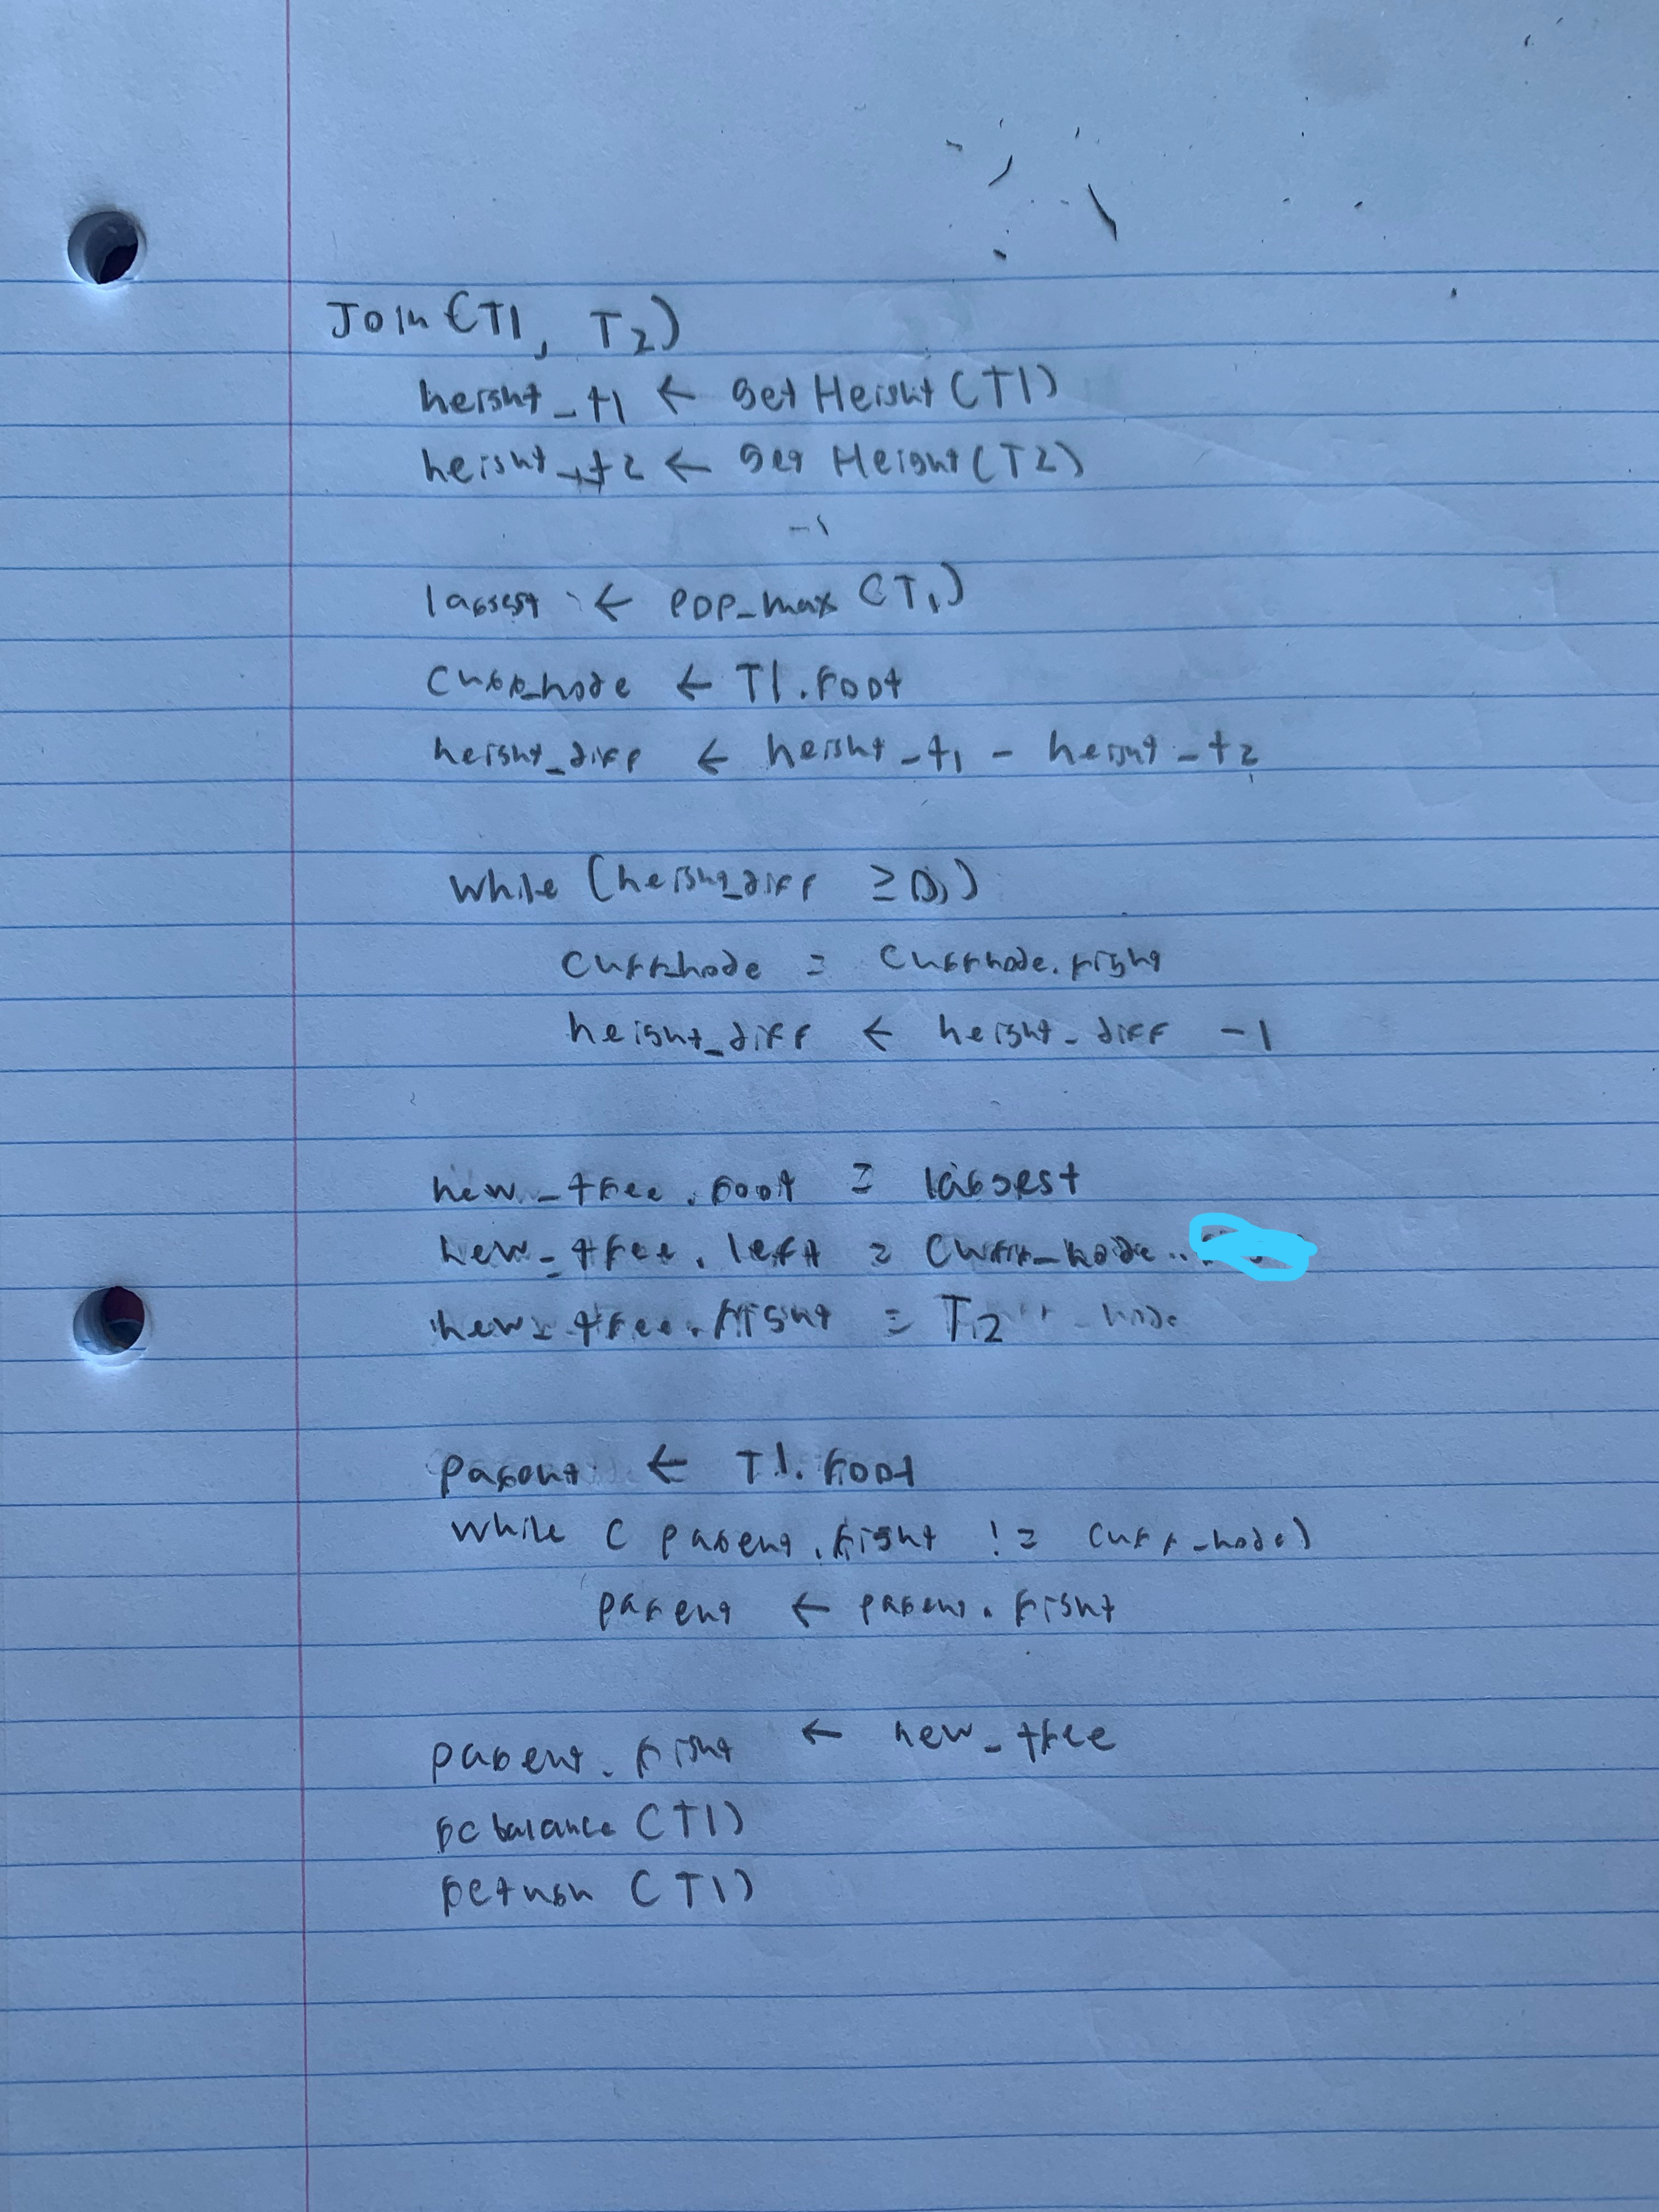
\includegraphics[width=0.7\textwidth, angle=0]{1.jpg}
	\end{center}
    \caption{Pseudocode for Join(T1, T2)}
	\label{figcaption}
\end{figure}
\end{adjustwidth} 
\newpage
\begin{adjustwidth}{0em}{0pt}
To begin we are going to get the heights of both T1 and T2, we will store these values inside height$\_$t1 and height$\_$t2. Since we are told that T1 has more nodes then T2 (and that all the values in T1 are smaller then those in T2) we will use the height later on to a node in T1 whose subtree is of an equal size as T2. [ Getting the heights will take O(height$\_$t1 + height$\_$t2) time ]\\ \\
Before we do this however we are going to find delete the largest value in T1 (which we know will be smaller then all the value values in T2). Then we will traverse down to the right of T1 using a variable called curr$\_$node which will find the height$\_$t1 - height$\_$t2 right most child. [ popping and storing the largest value in T1 will take O(log(T1)) time, traversing T1 will also take O(log(T1)) time ] \\ \\
Now the curr$\_$node will have a subtree with a height equal to T2, we will now create a new tree, using the largest value we stored at the start as the root (called variable largest). This root will be smaller then all values in T2 and larger then all values in curr$\_$node subtree. Thus we will make the left side of the tree equal to curr$\_$node and the right side equal to T2. [ Creating a new tree will take O(1) ]  \\ \\
We will then get the parent of current$\_$node and from there add the new tree to the right side of it. We will then iterate up from the parent and balance the tree. [getting the parent will take O(log(T1)) time, and balancing the tree will take O(log(newTree))] \\ \\
Therefore our total time complexity will be:
\[ O(height\_t1 + height \_ t2) + O(log(T1)) + O(log(T1)) + O(1) +  O(log(newTree)) \in O(log(newTree) \]
Which is the result as required


\end{adjustwidth} 
\end{document}